\documentclass{article}
\usepackage{fontspec}\defaultfontfeatures{Ligatures=TeX}
\usepackage{setspace}\setstretch{1.3} % \begin{spacing}{1.3}
\usepackage[a4paper,vmargin={1.5cm,2.5cm},hmargin={1.5cm,1.5cm}]{geometry}
%-----------------------------------------------------------------------------%
\usepackage{settings}
%-----------------------------------------------------------------------------%
%%% Title %%%
\title{一個關於剪紙的定理}
\author{\href{https://jessekelighine.com}{jessekelighine.com}\\Jesse C.\ Chen\ 陳\,捷}
\date{\texttt{\today}}
%-----------------------------------------------------------------------------%

\begin{document}
\begin{multicols}{2}

\begin{spacing}{1}
	\maketitle\thispagestyle{fancy}
\end{spacing}

\noindent
大家可能都有玩過七巧板,
能夠把原本拼成正方形的七塊拼圖拼成各式各樣的圖形。
類似的圖形拼貼謎題也很常見,
其中一個非常有名的便是 Henry Dudeney 在他 1907 年《The Canterbury Puzzles》書中提到\underdot{把正方形切割並拼貼成正三角形}的謎題
(這個謎題被稱為 Haberdaher's Problem)。
\begin{center}
	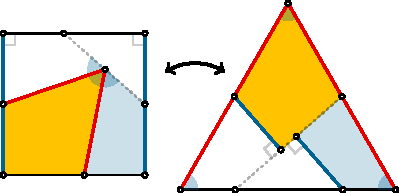
\includegraphics[scale=1]{figures/figure-example.pdf}
\end{center}
這些謎題都非常有趣,
但是能不能把這些謎題都一次解決呢?
也就是說,我們想要知道:
\begin{question*}
	能夠只透過有\underdot{限次}的剪剪貼貼,
	就把任意的圖形變成另一個面積相同的圖形嗎?
\end{question*}
\noindent
這個問題看似直接簡單,但又沒辦法直觀地說明對錯。
其實,這個問題的答案是肯定的,
並且只需要用基礎的幾何學知識就可以證明。
我們接下來就用歐幾里德式的證明來解決這麼問題吧!
% 你能想出要怎麼證明嗎?

\dinkus

\noindent
在開始之前,我們先清楚的定義所謂的\underdot{圖形}以及\underdot{剪貼}指涉的是什麼。

\begin{definition}[圖形]
	一個\textbf{圖形}指的是一個\underdot{簡單多邊形},
	也就是一個沒有洞,
	其邊不與自己相交,
	並且只有有限個角與邊的多邊形。
\end{definition}

\begin{definition}[剪貼]
	\textbf{剪}指將一個圖形以一條\underdot{直線分割}成兩部分。
	\textbf{貼}指的是把兩個圖形\underdot{不重疊地}合併再一起。
	\textbf{剪貼}指的是對一個圖形先進行數個\underdot{剪},
	後執行數個\underdot{貼},
	最後產生一個圖形且沒有剩餘的塊。
\end{definition}

\begin{remark}
	% 這些定義清楚地描述了我們討論的\underdot{圖形}是什麼,
	% 因為顯然地,只透過\underdot{剪貼}就想要把一個圓變成一個正方形是不可能的。
	簡單來說,一個\underdot{圖形}就是可以用直尺畫出來且沒有洞的形狀。
	而\underdot{剪貼}的定義就是一把剪刀剪下去再和在一起的概念。
	顯然地,任何一個圖形的面積在\underdot{剪貼}前後不會改變。
\end{remark}

\begin{theorem}\label{thm:reversible}
	如果一圖形 $A$ 能被剪貼成圖形 $B$,
	則圖形 $B$ 也能被剪貼成圖形 $A$。
\end{theorem}
\begin{proof}
	只要將剪貼的過程倒過來執行就可以了。
\end{proof}

\begin{theorem}\label{thm:triangulate}
	任何圖形可以被分割為有限個三角形。
\end{theorem}
\begin{proof}
	我們證明一個 $n$ 邊形可以被分割成 $n-2$ 個小三角形。
	我們用數學歸納法證明:
	\begin{center}
		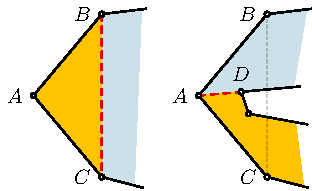
\includegraphics[scale=1]{figures/figure-triangulate.pdf}
	\end{center}
	\begin{itemize}
		\item[\underdot{起始}]
			當 $n=3$ 的時候,不需要分割就是個三角形。
		\item[\underdot{推遞}]
			當 $n\geq3$ 的時候,
			選取一頂點 $A$,
			其有兩個相鄰的頂點 $B$、 $C$。
			如果連線 $\overline{BC}$ 完全落在這個多邊形裡面,
			則把 $A$ 點去掉便成了一個 $n-1$ 邊形。
			根據歸納假設,這個 $n-1$ 邊形可以被分成 $n-3$ 個三角形。
			再把 $\triangle{ABC}$ 加上,那麼原本的 $n$ 邊形就能被分割成 $n-2$ 個三角形。
			那如果連線 $\overline{BC}$ 不完全落在這個 $n$ 邊形內部,
			則選取離 $\overline{BC}$ 最遠的頂點 $D$,
			連線 $\overline{AD}$ 必然完全落在這個 $n$ 邊形內部。
			連結 $\overline{AD}$ 便將原本的 $n$ 邊形分成兩個小多邊形,
			而兩個多邊形的頂點數 $m$ 與 $p$ 的和為 $n+2$。
			根據歸納假設,$m$ 邊形能被分為 $m-2$ 個三角形,
			$p$ 邊形能被分為 $p-2$ 個三角形,
			兩者相加得
			\begin{align*}
				(m-2) + (p-2)
				&= (m+p) -4 \\
				&= (n+2) -4
				= n-2。
			\end{align*}
			故 $n$ 邊形能被分割為 $n-2$ 個三角形。
			\qedhere
	\end{itemize}
\end{proof}

\begin{remark}
	雖然\textbf{\autoref{thm:reversible}} 以及\textbf{\autoref{thm:triangulate}} 看似無聊至極,
	但是對於等一下的證明非常重要,
	所以特別給他定理編號。
	另外,其實這兩個定理要能成立需要一個假設,
	那就是剪貼的過程要\underdot{有限}。
	這是為什麼我們一開始需要定義簡單多邊形。
\end{remark}

\begin{theorem}\label{thm:triangle-to-rectangle}
	任何三角形可以剪貼成長方形。
\end{theorem}
\begin{proof}
	考慮以下的圖形:
	\begin{center}
		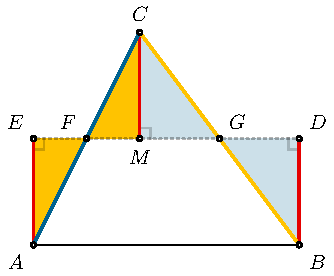
\includegraphics[scale=1]{figures/figure-triangle_to_rectangle.pdf}
	\end{center}
	我們想將 $\triangle{ABC}$ 剪貼成 $\square{ABDE}$。作法如下:
	\begin{enumerate}
		\item 令 $F$ 為 $\overline{AC}$ 的中點,並令 $G$ 為 $\overline{BC}$ 的中點;
		\item 令 $M$ 為 $C$ 在 $\overline{FG}$ 上的垂足;
		\item 將 $\triangle{ABC}$ 沿著 $\overline{FG}$ 以及 $\overline{CM}$ 剪開;
		\item 將 $\triangle{CFM}$ 旋轉 $180\degree$ 貼到 $\triangle{AFE}$ 的位置;
		\item 將 $\triangle{CMG}$ 旋轉 $180\degree$ 貼到 $\triangle{BDG}$ 的位置。
	\end{enumerate}
	我們宣稱通過這個作法剪貼成的 $\square{ABDE}$ 是一個與 $\triangle{ABC}$ 面積相同的長方形。

	首先,
	因為 $F$ 與 $G$ 分別是 $\overline{AC}$ 與 $\overline{BC}$ 的中點,
	我們知道以下三件事:
	\begin{itemize}
		\item $\blue{\overline{AF}}=\blue{\overline{CF}}$ 以及 $\yellow{\overline{CG}}=\yellow{\overline{BG}}$;
		\item $\overline{ED}$($\overline{FG}$ 的延伸)與 $\overline{AB}$ 平行;
		\item $\red{\overline{AE}}$、$\red{\overline{CM}}$ 與 $\red{\overline{BD}}$ 等長。
	\end{itemize}
	再來,注意到 $\triangle{CFM}\cong\triangle{AFE}$。
	這是因為 $\angle{CMF}=\angle{AEF}=90\degree$,
	斜邊 $\blue{\overline{AF}}=\blue{\overline{CF}}$,
	並且鄰邊 $\red{\overline{CM}}=\red{\overline{AE}}$,
	故 $\triangle{CFM}$ 與 $\triangle{AFE}$ 透過 RHS 全等。
	類似地,$\triangle{CMG}\cong\triangle{BDG}$,
	因為 $\angle{GMC}=\angle{GDB}=90\degree$,
	斜邊 $\yellow{\overline{CG}}=\yellow{\overline{BG}}$,
	以及鄰邊 $\red{\overline{CM}}=\red{\overline{BD}}$。
	因此,將 $\triangle{CFM}$ 以及 $\triangle{CMG}$ 分別貼到 $\triangle{AEF}$ 與 $\triangle{BDG}$ 的位置是可行的。

	最後,我們確認 $\square{ABDE}$ 是一個長方形。
	顯然的,因為 $\overline{ED}$ 與 $\overline{AB}$ 平行,
	並且 $\red{\overline{AE}}$ 與 $\red{\overline{BD}}$ 都和 $\overline{ED}$ 垂直,
	所以 $\square{ABDE}$ 是長方形。
\end{proof}

\begin{remark}
	如果 $\angle{BAC}$ 是直角,那麼我們在證明中使用的剪貼做法需要修改嗎?
	如果 $\angle{BAC}$ 是鈍角呢?
\end{remark}

\begin{theorem}\label{thm:rectangle-to-square}
	任何長方形可以剪接成正方形。
\end{theorem}
\begin{proof}
	考慮以下的圖形:
	\begin{center}
		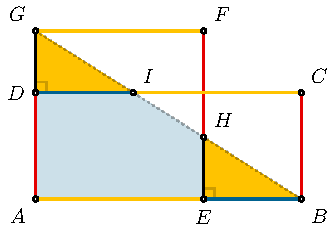
\includegraphics[scale=1]{figures/figure-rectangle_to_square.pdf}
	\end{center}
	我們想將 $\square{ABCD}$ 剪貼成正方形 $\square{AEFG}$。
	作法如下:
	\begin{enumerate}
		\item 將 $\yellow{\overline{AE}}$ 的長度定為 $\sqrt{\overline{AB}\cdot\red{\overline{BC}}}$;
		\item 令 $\yellow{\overline{CI}}=\yellow{\overline{AE}}$;
		\item 令 $H$ 為 $\overline{BI}$ 與 $\overline{AB}$ 在 $E$ 點垂線的交點;
			% \item 將 $I$ 定為與 $C$ 距離為 $\yellow{\overline{AE}}$ 的點,意即,$\yellow{\overline{CI}}=\yellow{\overline{AE}}$;
		\item 將 $\square{ABCD}$ 沿著 $\overline{BI}$ 以及 $\overline{EH}$ 剪開;
		\item 將 $\triangle{BCI}$ 平移貼到 $\triangle{HFG}$ 的位置;%,意即,讓 $\red{\overline{BC}}$ 與 $\overline{EH}$ 切齊;
		\item 將 $\triangle{BHE}$ 平移貼到 $\triangle{IGD}$ 的位置。
	\end{enumerate}
	我們宣稱通過這個作法剪貼成的 $\square{AEFG}$ 是與 $\square{ABCD}$ 面積相等的正方形。

	顯然地,
	將 $\triangle{BCI}$ 貼到 $\triangle{HFG}$ 的位置後,
	$\red{\overline{BC}}$ 與 $\overline{EH}$ 切齊並且
	$\overline{AG}$ 與 $\overline{AD}$ 共線。
	是故,我們只需說明 $\triangle{BHE}\cong\triangle{IGD}$ 並且確認 $\square{AEFG}$ 是正方形即可完成證明。

	注意到因為 $\yellow{\overline{AE}}=\yellow{\overline{CI}}$,所以 $\blue{\overline{BE}}=\blue{\overline{DI}}$;
	又因為 $\red{\overline{FH}}=\red{\overline{AD}}$,所以 $\overline{EH}=\overline{DG}$;
	最後因為 $\angle{BEH}=\angle{IDG}=90\degree$,
	故 $\triangle{BHE}$ 與 $\triangle{IGD}$ 因為 SAS 全等。
	因此,將 $\triangle{BHE}$ 貼到 $\triangle{IGD}$ 的位置之後 $\square{AEFG}$ 便是一個完整的長方形。

	最後我們確認 $\square{AEFG}$ 其實是一個正方形。
	這是顯然的,
	因為 $\square{AEFG}$ 與 $\square{ABCD}$ 面積相同,
	又因為 $\yellow{\overline{AE}}$ 的長度是 $\sqrt{\overline{AB}\cdot\red{\overline{BC}}}$,
	所以我們必然有 $\yellow{\overline{AE}}=\red{\overline{FH}}+\overline{EH}$。
\end{proof}

\begin{remark}
	在以上的證明中,
	我們說:
	\begin{quote}
		顯然地,
		將 $\triangle{BCI}$ 貼到 $\triangle{HFG}$ 的位置後,
		$\red{\overline{BC}}$ 與 $\overline{EH}$ 切齊並且
		$\overline{AG}$ 與 $\overline{AD}$ 共線。
	\end{quote}
	這件事看圖的確是顯然的,但是我們沒有提供嚴謹的證明。
	如果 $\square{ABCD}$ 是一個長寬比為 $5:1$ 的長方形,
	那以上的這個\underdot{顯然}的事實還成立嗎?
	如果不成立,遇到的問題是什麼?然後要怎麼修改證明中使用的作法呢?
\end{remark}

\begin{theorem}\label{thm:pythagorean}
	任兩個正方形可以剪貼成一個正方形。
\end{theorem}
\begin{proof}
	考慮以下的圖形:
	\begin{center}
		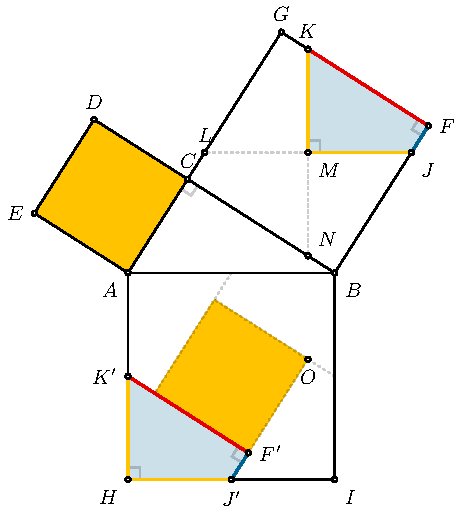
\includegraphics[scale=1]{figures/figure-pythagorean.pdf}
	\end{center}
	我們想將 $\square{ACDE}$ 與 $\square{BFGC}$ 合併成一個大的正方形 $\square{AHIB}$。
	作法如下:
	\begin{enumerate}
		\item 將 $\square{ACDE}$ 與 $\square{BFGC}$ 如圖放置在直角三角形 $\triangle{ABC}$ 的兩股;
		\item 令 $M$ 為 $\square{BFGC}$ 的中點;
		\item 令 $\overline{KN}$ 為過 $M$ 且與 $\overline{AB}$ 垂直的線段;
		\item 令 $\overline{LJ}$ 為過 $M$ 且與 $\overline{AB}$ 平行的線段;
		\item 將 $\square{BFGC}$ 沿著 $\overline{KN}$ 以及 $\overline{LJ}$ 剪開;
		\item 將 $\square{ACDE}$ 與 $\square{KMJF}$ 等四塊四邊形如圖照虛線平移並貼成 $\square{AHIB}$。
	\end{enumerate}
	我們宣稱通過這個作法剪貼成的正方形 $\square{AHIB}$ 的面積等於 $\square{ABCD}$ 及 $\square{BFGC}$ 面積的總和。

	首先,由於 $\overline{LJ}$ 平行於 $\overline{AB}$,
	並且 $\overline{AL}$ 平行於 $\overline{BJ}$,
	$\square{ABJL}$ 是一個平行四邊形。
	另外,由於 $M$ 是 $\square{BFGC}$ 的中心點,
	故 $\yellow{\overline{MJ}}$、$\yellow{\overline{MK}}$ 與 $\overline{ML}$ 等長。
	因此,$\yellow{\overline{MK}}=\yellow{\overline{MJ}}$ 是 $\overline{AB}$ 長度的一半,
	並且 $K'$ 與 $J'$ 分別是 $\overline{AH}$ 與 $\overline{HI}$ 的中點。
	又因為 $\blue{\overline{FJ}}$ 平行於 $\overline{GL}$,$\red{\overline{FK}}$ 平行於 $\overline{BN}$⋯等平行關係,
	從 $\square{BFGC}$ 剪出來的四塊四邊形可以緊密的貼到 $\square{AHIB}$ 中的四個角落。

	最後,我們說明 $\square{BFGC}$ 中間就剩下的正方形洞的面積恰好就是與 $\square{ACDE}$ 的面積相等。
	再次注意到平行四邊形 $\square{ABJC}$,可以發現 $\square{ACDE}$ 的邊長恰好是
	\begin{align*}
		\overline{AC}
		= \overline{AL} - \overline{CL}
		= \overline{JB} - \overline{CL}
		= \red{\overline{FK}} - \blue{\overline{FJ}},
	\end{align*}
	而 $\square{BFGC}$ 中間就剩下的正方形洞的邊長是
	\begin{align*}
		\overline{F'O}
		= \overline{J'O} - \blue{\overline{F'J'}}
		= \red{\overline{F'K'}} - \blue{\overline{F'J'}}。
	\end{align*}
	是故,$\square{ACDE}$ 可以完美地鑲嵌在 $\square{BFGC}$ 中間就剩下的正方形洞中。
\end{proof}

\begin{remark}
	\textbf{\autoref{thm:pythagorean}} 的證明就是勾股定理的一種證明,
	而我們證明方式是直接建構將兩個小正方形\underdot{剪貼}成大正方形的作法。
	其實,只使用\textbf{\autoref{thm:reversible}} 以及\textbf{\autoref{thm:rectangle-to-square}}
	也能建構出將兩個小正方形合併成一個大正方形的作法。
	你能想出是什麼作法嗎?
\end{remark}

\begin{theorem}[Wallace-Bolyai-Gerwien]\label{thm:WBG}
	任何一個圖形都可以剪貼成任一個面積相同的圖形。
\end{theorem}
\begin{proof}
	假設有兩個面積相同的圖形 $A$ 和圖形 $B$。
	根據\textbf{\autoref{thm:triangulate}},
	先將 $A$ 分成數個三角形。
	再根據\textbf{\autoref{thm:triangle-to-rectangle}} 以及\textbf{\autoref{thm:rectangle-to-square}},
	將所有三角形都先剪貼成長方形,再剪貼成正方形。
	最後根據\textbf{\autoref{thm:pythagorean}}
	把所有小正方形合併成一個面積與 $A$ 相等的大正方形。
	同理,圖形 $B$ 也可以通過一樣的方法被剪貼成一個面積相等的大正方形。
	是故,
	先將圖形 $A$ 剪貼成大正方形,
	再根據\textbf{\autoref{thm:reversible}},
	就能將大正方形剪貼成圖形 $B$。
\end{proof}

\noindent
如此一來,我們一開始的問題就就靠著\textbf{\autoref{thm:WBG}} 解決了!

\dinkus

\noindent
最後這個定理被稱為 Wallace-Bolyai-Gerwien Theorem,
因為有三位數學家各自在 19 世紀初獨立地證明了這個定理,
所以這個定理就冠上這三位數學家的名字。

從一開始 Henry Dudeney 的例子可見,
我們的證明方法顯然在很多情況下是太費工了。
可以說我們給的剪貼次數是一個\underdot{上界},
也就是說:
必定可以使用我們提供的剪貼程序完成圖形之間的轉換,
但是在很多時候可以通過更簡易的程序完成剪貼。
而找尋這些更簡易的程序也就是這些謎題的有趣之處。
一開始我們給出了 Henry Dudeney 把正方形剪貼成正三角形的作法,
但是沒有給出尺寸的細節。
你能夠\underdot{看圖}用\underdot{尺規作圖}建構出 Henry Dudeney 切割正方形或正三角形的方法嗎?
\asDemonstrated

\end{multicols}

\noindent
\begin{turn}{180}
	\begin{solution*}
		要能夠直想出這樣的切割方式不簡單,
		但是有一開始的圖要反推剪貼方式就要簡單得多。
		首先,觀察到 $\blue{\overline{AM}}=\blue{\overline{DM}}$ 並且 $\blue{\overline{BE}}=\blue{\overline{CE}}$,
		這是因為這四個邊在貼成正三角形時要兩兩重合。
		類似地,$\red{\overline{MN}}=\red{\overline{NO}}=\red{\overline{EL}}$。
		接著,因為正方形與正三角形面積相等,所以
		$4\cdot\blue{\overline{AM}}^2 = \sqrt{3}\cdot\red{\overline{MN}}^2$,
		這就表示
		$\red{\overline{MN}} = \frac{2}{\sqrt[4]{3}} \blue{\overline{AM}}$。
		有了這些關係就可以開始尺規作圖了。
		為了方便起見,在尺規作圖中令 $\blue{\overline{AM}}=1$:\\
		\begin{minipage}{0.58\textwidth}
			\begin{enumerate}
				\item 令 $C'$ 使得 $\overline{BC'}=\overline{BC}$ 並以 $B$ 為圓心作半圓 $\overarc{C'C}$;
				\item 令過 $E$ 點 $\overline{BC}$ 垂線交半圓 $\overarc{C'C}$ 於 $F$;
				\item 令 $G$ 使得 $\overline{EG}=\overline{CE}$ 並以 $\overline{FG}$ 為直徑做半圓 $\overarc{FG}$;
				\item 令 $\overline{CE}$ 之延伸交 $\overarc{FG}$ 於 $I$(此時 $\overline{EI}=\sqrt[4]{3}$);
				\item 令 $J$ 為過 $C$ 且與 $\overline{GI}$ 平行之線之交點(此時 $\overline{EJ}=1/\sqrt[4]{3}$);
				\item 以 $J$ 為圓心 $\overline{EJ}$ 為半徑作半圓 $\overarc{EK}$(此時 $\overline{EK}=2/\sqrt[4]{3}$);
				\item 以 $E$ 為圓心 $\overline{EK}$ 為半徑作弧交 $\overline{CD}$ 於 $L$;
				\item 以 $M$ 為圓心 $\overline{EK}$ 為半徑作弧交 $\overline{EL}$ 於 $N$;
				\item 以 $N$ 為圓心 $\overline{EK}$ 為半徑作弧交 $\overline{AB}$ 於 $O$。
			\end{enumerate}
		\end{minipage}
		\begin{minipage}{0.35\textwidth}
			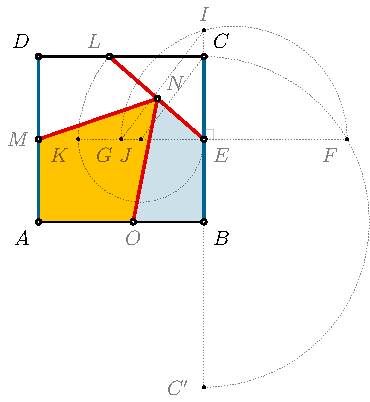
\includegraphics[scale=1]{figures/figure-example_construction.pdf}
		\end{minipage}\\
		最後,
		請再驗證這樣尺規作圖出來的切割方式真的可以被拼剪成一個正三角形。
		\asDemonstrated
	\end{solution*}
\end{turn}

\end{document}
